\graphicspath{{./Linear_PDEs/}}

\section{Linear PDEs}

In this section we will illustrate how to solve some linear partial differential equations, \emph{PDEs}. Namely we will discuss how to use
\begin{enumerate}
\item Classification of PDEs
\item Derivations of classical linear PDEs
\item Method of Characteristics
\item Separation of Variables
\item Fourier Transforms / Laplace Transforms
\item Similarity Solutions
\item Method of Images
\end{enumerate}

to solve various kinds of {\bf{linear}} PDEs. Solutions to non-linear PDEs are not very friendly to the ole paper and pencil formulations that we love, cherish, and admire. First we begin by classifying equations. To do so, let's state what we mean by linear PDEs! We will illustrate this using $2^{nd}$ order PDEs, as a lot of natural phenomena is successfully mathematically modeled using $2^{nd}$ order PDE operators, but that is a story for another day. \\

We consider a function $u=u(x,y)$, that is a function of N independent variables, and write the general form of a $2^{nd}$ order linear PDE as,
\begin{equation}
\label{2nd_order_pde} A \frac{ \partial^2 u}{\partial x^2} + B \frac{ \partial^2 u}{\partial x\partial y} + C \frac{ \partial^2 u}{\partial y^2} + D \frac{\partial u}{\partial x} + E \frac{\partial u}{\partial y} + Fu = G(x,y),
\end{equation}

where $A,B,C,D,E,F$ and $G$ are functions of $x$ and $y$. As in ordinary differential equations, if $G(x,y)=0$ the PDE is said to be \emph{homogeneous}, otherwise it is said to be \emph{non-homogeneous}.\\

Fortunately we are able to classify different types of PDEs, which give rise to solutions with radically different behavior, using the coefficient functions $\{A,B,C,\ldots,F\}$. Furthermore in the case when $\{A,B,C,D,E,F\}$ are constants, i.e., the PDE has constant coefficients, when we classify a PDE there is no possibility of changing types spatially (or temporally). We classify them using the following, 
\begin{enumerate}
\item {\bf{Hyperbolic}}: $B^2 - 4AC > 0$
\item {\bf{Parabolic}}: $B^2 - 4AC = 0$
\item {\bf{Elliptic}}: $B^2 - 4AC < 0$
\end{enumerate}

In a nutshell, the classification of $2^{nd}$ order PDEs is very important, but is beyond the scope of what we wish to discuss here. We will note that the classification helps give rise to certain kinds of boundary conditions and/or initial conditions for a PDE. Furthermore we will say that \emph{hyperbolic} equations are related to wave phenomena, \emph{parabolic} are related to dissipative processes and heat flow, and \emph{elliptic} equations are related to steady-states of a system.\\

In the case of $1^{st}$ Order Systems of PDEs, we can classify the system based on properties of the coefficient matrices, $A$ and $B$, where our general equation is of the form,
$$A{\bf{u}}_t + B{\bf{u}}_x = {\bf{c}}.$$

Depending on the invertibility of $A$ or $B$, we \emph{may or may not} be able to classify the system as elliptic, hyperbolic, or parabolic. If $A$ is non-singular, and $B$ may or may not be, we consider the problem of 
\begin{align*}
\mbox{Eigenvalues}&: det(B-\lambda A) = 0 \\
\mbox{Eigenvectors}&: (B-\lambda A){\bf{v}} = 0. \\
\end{align*}

However, if the opposite situation arises, where $B$ is known to be non-singular, and $A$ may or may not be, we consider the analogous problem of
\begin{align*}
\mbox{Eigenvalues}&: det(A-\lambda B) = 0 \\
\mbox{Eigenvectors}&: (A-\lambda B){\bf{v}} = 0. \\
\end{align*}

We then have the following three cases, depending on what the eigenvalues are found to be:
\begin{itemize}
\item[] {\bf{Elliptic}}: No real eigenvalues $\Rightarrow$ eigenvalues are \emph{strictly complex} with $Im\neq 0$. ($\#$ of eqns. must be even!)
\item[] {\bf{Hyperbolic}}: $N$ real eigenvalues and yield a full set of linearly independent eigenvectors
\begin{itemize}
\item a. $N$ real \emph{distinct} eigenvalues $\Rightarrow$ $N$ linearly independent eigenvectors
\item b. Repeated eigenvalues may or may not yield a full set of linearly independent eigenvectors (if full set, only then is the system hyperbolic).
\end{itemize}
\item[] {\bf{Parabolic}}:  $N$ real eigenvalues, which do \emph{not} yield a full set of linearly independent eigenvectors. This can only occur if there are repeated eigenvalues.
\end{itemize}

We will just a few more notes of classification of these $1^{st}$ order PDE systems.  \emph{Note:}
\begin{enumerate}
\item You cannot classify a system if it has both real and complex eigenvalues
\item Since in general $A=A(x,t,{\bf{u}})$ and $B=B(x,t,{\bf{u}})$ $\Rightarrow \lambda = \lambda(x,t,{\bf{u}})$ and therefore classification can vary from point to point in the $(x,t)$-plane.
\item For the scalar equation $$a(x,t,u) u_t + b(x,t,u) u_x = c(x,t,u),$$
we have $$\lambda = \frac{b(x,t,u)}{a(x,t,u)}\ \ \mbox{ or } \ \ \lambda = \frac{a(x,t,u)}{b(x,t,u)},$$ 
and hence only have \emph{one} real distinct eigenvalue. Therefore a scalar $1^{st}$ order PDE is always hyperbolic!
\end{enumerate}


Actually before proceeding further, let's take that dive and derive some of those more popular $2^{nd}$ order PDEs that everyone is ranting and raving about, namely the wave equation, heat equation, and Laplace's equation.\\

Let's start off with the \emph{wave equation}! (and surf along from there...) \\ \\ 

%
% Begin Deriving PDE Section
%
%\begin{itemize}
\subsection{Quick derivations of the big three - elliptic, hyperbolic, and parabolic PDEs.}

In this section we will motivate the phenomena in which where the \emph{wave equation} (hyperbolic) and \emph{heat equation} (parabolic) PDEs govern the behavior. Furthermore we will also briefly build up intuition behind \emph{Laplace's Equation} (elliptic); however, we will not derive it. 

%
%WAVE EQUATION
%
%\item[] {\bf{WAVE EQUATION}}: $$u_{tt} = a^2 u_{xx}$$
\subsubsection{Derivation of the Wave Equation:} $$u_{tt} = a^2 u_{xx}$$

Consider a guitar string of length $L$, that is tethered at two ends along the $x$-axis, say at $x=0$ and $x=L.$ When one plucks the string, we assume the all vibrational motion takes place perpendicular to the $x$-axis, e.g., transverse vibrations. We will let $u=u(x,t)$ denote the vertical displacement of the string at any point $x\in(0,L)$ for $t>0$.\\

To derive the wave equation, we will need to make a few simplifying assumptions about the material properties of the string and problem at hand. We will assume
\begin{enumerate}
\item The string is flexible and has no preferred shape
\item The string is homogeneous, i.e., the mass per unit length, $\rho$, is constant
\item The displacements are small compared to the length of the string, e.g.,  $u(x,t)<<L$
\item From above, we get that this implies the slope of the string's curvature is small at all points $x\in(0,L)$
\item The string's tension acts tangent to the string and magnitude is constant among all points on the string
\item The tension defeats the force of gravity entirely, i.e., ignore it. It's weak...unless this is the guitar near the event horizon of a black hole.
\item Actually, let's assume no external forces are present. No electromagnetic force. No nuclear forces. No gravity. (This is still better than spherical cows.)
\end{enumerate}

We consider a small interval on the string $[x_j,x_j+\Delta x]$. The tensions on the end of this interval are, of course, tangent to the ends of the curved string. We next proceed by computing the net vertical force on the string, in hopes of employing Newton's second law of motion to giving us our model. Assuming small angular displacements, we compute the force acting on the element $\Delta s$ (it's small, I swear!) and obtain
\begin{align*}
T \sin\theta_2 - T\sin\theta_1 &\approx T\tan\theta_2 - T\tan\theta_1 \\
&= T\left[ \frac{\partial u}{\partial x}\Big|_{(x_j+\Delta x, t)}  \right] - T\left[ \frac{\partial u}{\partial x}\Big|_{(x_j, t)}  \right]\\
&= T\left[ \frac{\partial u}{\partial x}\Big|_{(x_j+\Delta x, t)}  -  \frac{\partial u}{\partial x}\Big|_{(x_j, t)}  \right]
\end{align*}

since $ \frac{\partial u}{\partial x}\Big|_{(x_j+\Delta x, t)} = \tan\theta_2$ and $\frac{\partial u}{\partial x}\Big|_{(x_j, t)}  = \tan\theta_1$ from slope relationships. We also note that from our assumptions above $T=| {\bf{T}}_1 |= |{\bf{T}}_2|$.\\

Now that we know all the tensile forces acting on the string, we use the rest of Newton's second law of motion to relate it to the string's acceleration. We simply use the assumption that $$\rho \Delta s \approx \rho \Delta x,$$

to give us a fair approximation to the mass of the string on $[x_j,x_j+\Delta x]$. The acceleration term is then $\rho\Delta s \frac{\partial^2 u}{\partial t^2} = \rho\Delta x \frac{\partial^2 u}{\partial t^2}$. Hence Newton's second law gives us
$$\rho\Delta x \frac{\partial^2 u}{\partial t^2} =  T\left[ \frac{\partial u}{\partial x}\Big|_{(x_j+\Delta x, t)}  -  \frac{\partial u}{\partial x}\Big|_{(x_j, t)}    \right].$$

Next rearranging we get $$\frac{\partial^2 u}{\partial t^2} = \frac{T}{\rho} \frac{\frac{\partial u}{\partial x}\Big|_{(x_j+\Delta x, t)}  -  \frac{\partial u}{\partial x}\Big|_{(x_j, t)} }{\Delta x}.$$

Finally taking the limit as $\Delta \rightarrow 0$, we get the wave equation in all its linear glory,

$$\frac{\partial^2 u}{\partial t^2} = a^2 \frac{\partial^2 u}{\partial x^2},$$

where $a^2 = \frac{T}{\rho}.$ \\ \\

%
% Heat Equation
%
%\item[] {\bf{HEAT EQUATION}}: $$\frac{\partial u}{\partial t} = k \frac{\partial^2 u}{\partial x^2}$$
\subsubsection{Derivation of the Heat Equation:}  $$\frac{\partial u}{\partial t} = k \frac{\partial^2 u}{\partial x^2}$$

We consider a long, thin wire in which heat transfer occurs. We call $u(x,t)$ the temperature of the wire at position $x$ at time $t$. We consider only a thin (circular) rod, say it with length $L$. We will plop this wire down on the $x$-axis, and hence the wire lays on $x\in[0,L]$. If you'd like we can say the wire has cross-sectional area, A; however, we will find it won't matter in the long run!\\

Now come our simplifying assumptions!
\begin{enumerate}
\item The flow of heat only takes place within the metal rod, i.e., the rod is insulated
\item No heat is being generated within the rod, e.g. no source terms...yet!
\item The rod is homogeneous, e.g., the mass per unit volume $\rho$ is constant
\item The specific heat $\gamma$ and thermal conductivity $K$ of the material are constants (it gets more \emph{interesting} when they aren't, though)
\end{enumerate}

Now unlike the wave equation, where we simply used Newton's second law of motion to derive our model equation, we need to use two empirical laws in heat flow. These laws are very logical and may not seem like they deserve the title of being an empirical \emph{law}. 
\begin{enumerate}
\item The rate of heat flow through a cross-section, A, is proportional to the cross-sectional area and the partial derivative with respect to $x$ of the temperature:$$ \frac{dQ}{dt} = -KA\frac{\partial u}{\partial x}.$$ The minus sign is to ensure that heat flows from the higher to lower temperature direction. 

\item The quantity of heat, $Q$, at point $x$, within an element of mass m is $$Q=\gamma m u(x,t) = \gamma\rho A\Delta x u,$$
where $m = \rho(A\Delta x).$ We can now differentiate the above equation with respect to time to give us a heat flow rate, $$\frac{dQ}{dt} = \gamma\rho A\Delta x\frac{\partial u}{\partial t}.$$
\end{enumerate}

Now when heat is flowing in the positive $x$ direction, we see that heat will build up at a rate of $$-KA \frac{\partial u}{\partial x} \Big|_{(x,t)} - \left( -KA \frac{\partial u}{\partial x} \Big|_{(x+\Delta x,t)}  \right) = -KA\left[  \frac{\partial u}{\partial x} \Big|_{(x+\Delta x,t)}  - \frac{\partial u}{\partial x} \Big|_{(x,t)}  \right].$$

Hence equating this with our second empirically derived relation, gives $$\gamma\rho A \Delta \frac{\partial u}{\partial t} =  KA\left[   \frac{\partial u}{\partial x} \Big|_{(x+\Delta x,t)}  - \frac{\partial u}{\partial x} \Big|_{(x,t)}  \right],$$

and therefore

$$\frac{\partial u}{\partial t} =  \frac{K}{\gamma\rho} \frac{  \frac{\partial u}{\partial x} \Big|_{(x+\Delta x,t)}  - \frac{\partial u}{\partial x} \Big|_{(x,t)} }{\Delta x}.$$

Finally taking the limit as $\Delta x\rightarrow 0$, we obtain the heat equation, e.g., 

$$\frac{\partial u}{\partial t} = \kappa \frac{\partial^2 u}{\partial x^2},$$

where $\kappa = \frac{K}{\gamma\rho}.$


%\item[] {\bf{Laplace's Equation}}: $$\Delta u = \nabla^2 u = \frac{\partial^2 u}{\partial x^2} + \frac{\partial^2 u}{\partial y^2} = 0.$$
\subsubsection{Intuition about Laplace's Equation:}
$$\Delta u = \nabla^2 u = \frac{\partial^2 u}{\partial x^2} + \frac{\partial^2 u}{\partial y^2} = 0.$$

First we note that we will not derive Laplace's equation in this section. Sorry to disappoint you. Instead we will try to motivate it as well as give some physical insight to what the equation says, while also defining some operators. Let's start there. The Laplacian operator, which acts on \emph{Euclidiean n-space}, can be thought as the operator of non-mixed second partial derivatives with respect to the spatial variables. In $n$-dimensions the operator looks like 
\begin{equation}
\label{Laplacian} \Delta = \sum_{j=0}^{n} \frac{\partial ^2 }{\partial x_j^2} = \frac{\partial ^2 }{\partial x_1^2}  + \frac{\partial ^2 }{\partial x_2^2} +\ldots + \frac{\partial ^2 }{\partial x_n^2}.
\end{equation}

When we restrict ourselves to two spatial variables, say $x$ and $y$, it takes the form in the above Laplace Equation. It can also be thought of as the \emph{divergence} of the \emph{gradient} of a vector. It is not related to our other friend, the Laplace Transform. There are two ways we will build some intuition about the Laplacian. \\

In building intuition, let's start off with something we all know well - basic calculus. Remember back to your calculus 1 days, where taking a derivative was the answer to virtually everything, and sometimes you had to take a second derivative to check something. Well that \emph{something}, the \emph{concavity} is where we begin. \\

Recall if we have a function $y=f(x)$ and $f''(x)<0$, then $y$ is concave up, while if $f''(x)>0$, then $y$ is concave down. Analogously the Laplacian can be thought of as the generalization to multivariate functions.\\

Likewise, we could also think of the Laplacian as a ``local averaging operator". The Laplacian basically compares the value of $u$ at some point to all the points within a neighborhood of it. This can also, perhaps, give better insight into the concavity idea. There are three pathological cases, listed below. 
\begin{enumerate}
\item $\Delta u=0$: $u$ at a point is equal to its neighbors (Laplace's Equation)
\item $\Delta u>0$: $u$ at a point is less than the average of its neighbors
\item $\Delta u<0$: $u$ at a point is greater than the average of its neighbors
\end{enumerate}

Hence we have the idea that $$\Delta u \approx ``\mbox{the average of all points in a neighborhood of }\  u \mbox{ at }\  \vec{x}."$$

Now when we think of say, the heat equation, which can be written as $$u_{t} = k \Delta u,$$

we can think of it as the rate of change with respect to time of the temperature is proportional to the difference between the average temperature of $u$ at a point and the value at the point itself. For example, if there is a very cold spot in our domain, the surrounding domain is warmer, and hence the Laplacian will be positive and thereby more heat will flow into that region, causing the temperature to rise in our once colder spot.\\

%\end{itemize} 
%
% End Deriving PDE Section
%

One last remark before we proceed with solution methodoglies to linear PDEs. We state that if $u_1,u_2,\ldots,u_k$ are solutions of a homogeneous linear PDE, then their linear combination $$u = \sum_{j=1}^{k} c_j u_k = c_1 u_1 + c_2 u_2 + \ldots + c_k u_k,$$ is also a solution, assuming $\{ c_j \}\in\mathbb{C}$. This is fondly known as the \emph{superposition principle}. Splendid. Time to rock!


%%%%%%%%%%%%%%%%%%%%%%%%%%%%%%%%%%%%%
%
% METHOD OF CHARACTERISTICS
%
%%%%%%%%%%%%%%%%%%%%%%%%%%%%%%%%%%%%%

\subsection{Method of Characteristics: For $1^{st}$ order linear PDE}

The basic mechanics behind the \emph{method of characteristics} transforms our problem from one of PDE nature into an ODE challenge. Characteristics themselves can be thought of as curves, in which the PDE reduces to an ODE. We now consider the following \emph{Cauchy problem},

$$a(x,y) u_x + b(x,y) u_y = c(x,y,u),$$ with initial corresponding initial data $u|_\mathscr{C} = u_0$, where $\mathscr{C}$ is some curve to which the initial data is defined. We also note that this type of $1^{st}$ order PDE is called \emph{quasi-linear} due to the non-homogeneous term, possibly being a nonlinear function of $u(x,y)$.\\

We will now motivate and build intuition on the method of characteristics.

\subsubsection{Conceptual Ideas:}

We will list the steps and motivate each behind the method now, upon considering the Cauchy problem described above.

\begin{enumerate}
\item Make a coordinate transformation: $(x,y) \rightarrow (\tau, s)$ so that
\begin{itemize}
\item[(i)] $\mathscr{C}$ corresponds to the $\tau$-axis ($s=0$), i.e., the level curves of $s(x,y)=0.$
\item[(ii)] We call the \emph{characteristics} of the PDE, the level curves, $\tau(x,y)=constant.$ The PDE will reduce to an ODE on these curves.
\end{itemize}

\item Along each level curve, $\tau(x,y)=constant$, the PDE reduces to an ODE. 

\item PDE is subject to prescribed $u$ on the parameterized initial data curve $$\mathscr{C}: \left. \begin{array}{c} x= f(\tau) \\ y = g(\tau) \end{array}\right\} \Rightarrow u=u(f(\tau),g(\tau)) = u_0(\tau).$$
\begin{itemize}
\item[(i)] Transform coordinates so that $(x,y)\rightarrow (\tau,s).$
\item[(ii)] This entails 
\begin{align*}
x = x(\tau,s) \ \ &\ \ \tau=\tau(x,y) \\
y = y(\tau,s) \ \ &\ \ s = s(x,y).
\end{align*}
\item[(iii)] Furthermore our initial data makes the constraints,
\begin{align*}
x(\tau,0) &= f(\tau) \\
y(\tau,0) &= g(\tau) \\
u(\tau,0) &= u_0(\tau). \\
\end{align*}
\end{itemize}

\begin{figure}[h!]
\centering
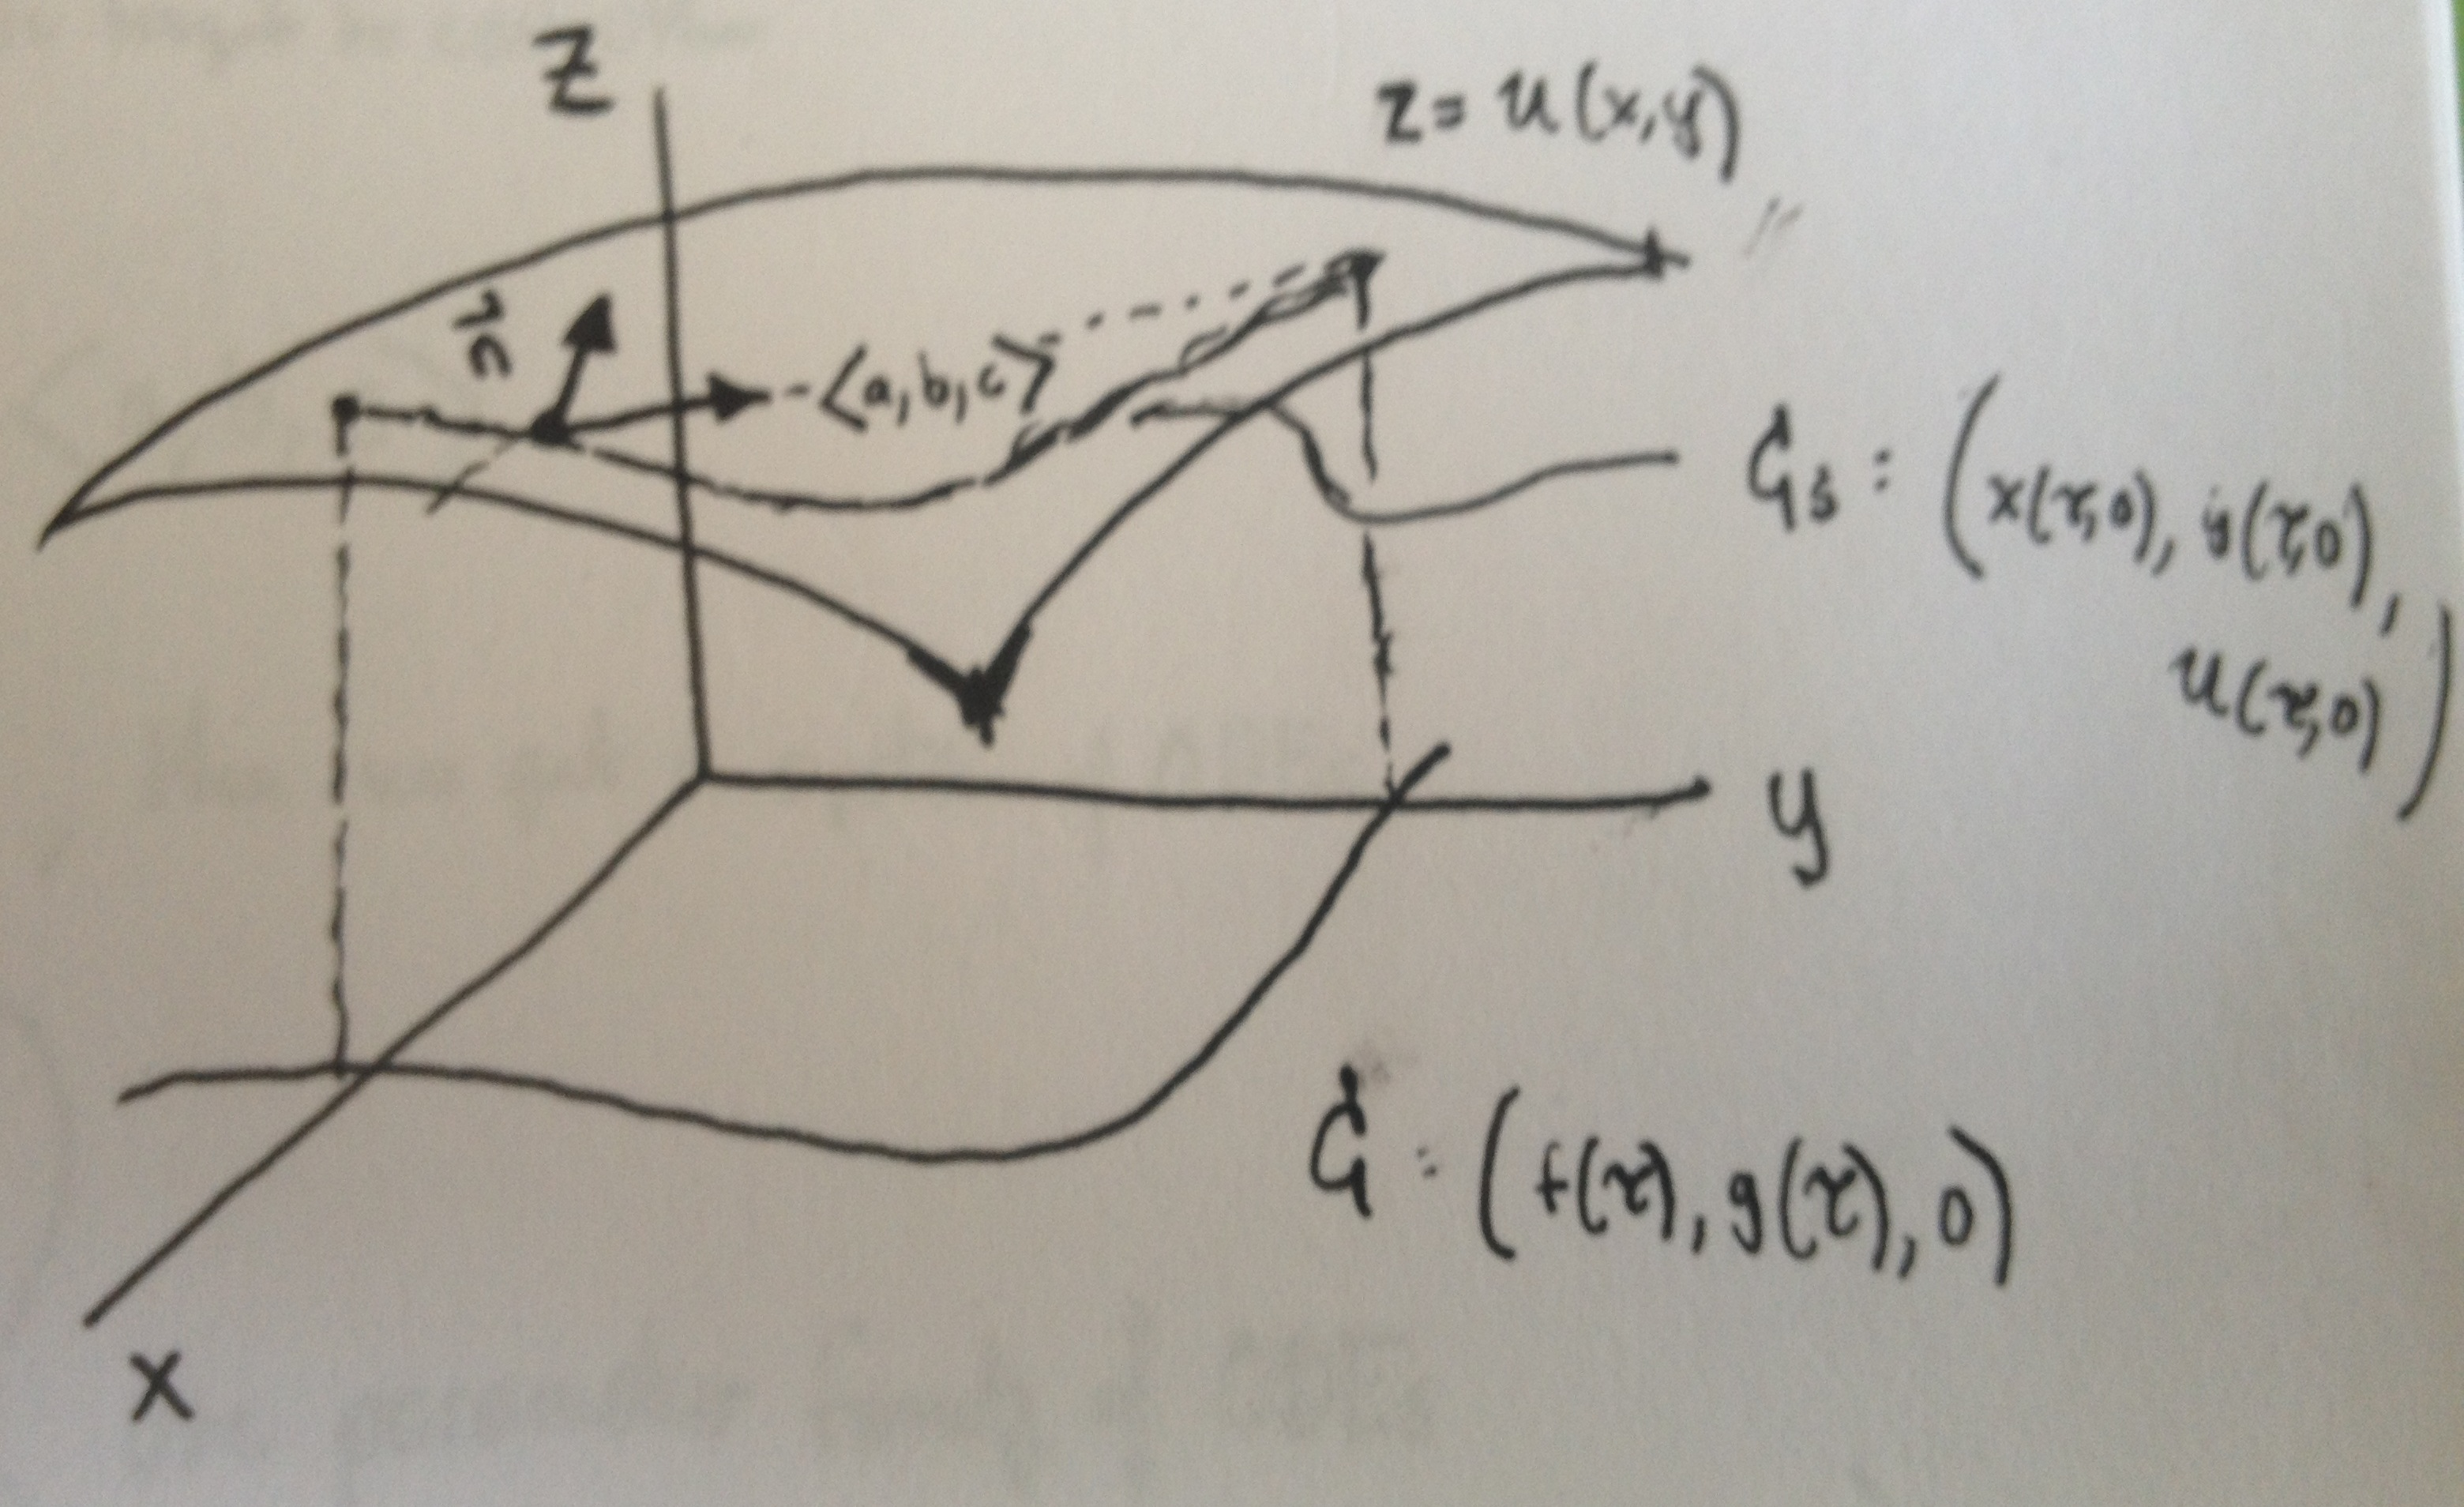
\includegraphics[width=3.0in]{moc_idea1.jpg}
\caption{General idea of the Cauchy problem's initial data.}
\label{moc_idea1}
\end{figure}

\item The solution is going to be a surface in $z=u(x,y)$ for the Cauchy problem which contains the initial data, $\mathscr{C}: (x(\tau,0), y(\tau,0), u(\tau,0)).$ This can be seen in Figure(\ref{moc_idea1}).\\

This surface can be thought of as a level curve of the function, $F(x,y,z) = u(x,y)-z=0,$\\

with corresponding normal vector, ${\bf{n}} = \nabla F = <u_x,u_y,-1>.$

Notice that the vector $<a,b,c>$ lies in the tangent plane of the solution surface at each point on it, e.g., $$<a,b,c>\cdot {\bf{n}} = <a,b,c>\cdot<u_x,u_y,-1> = au_x + bu_y - c = 0.$$

Following the vector $<a,b,c>$, it directs us along a curve on the solution surface. 
\begin{itemize}
\item[(i)] Such a curve passes through each point of the initial data curve, $\mathscr{C}_s$, given a one-parameter family of curves, with the parameter, $\tau$, specifying which one. 
\item[(ii)] Define $\tau$ so that it is constant along each curve, thus giving a one-parameter family of curves.  The curves are then the level curves of $\tau(x,y)=constant$.
\item[(iii)] Only $s$ varies along each curve, with $s=0$, corresponding to the points on the initial data curve, $\mathscr{C}_s$.

\begin{figure}[h!]
\centering
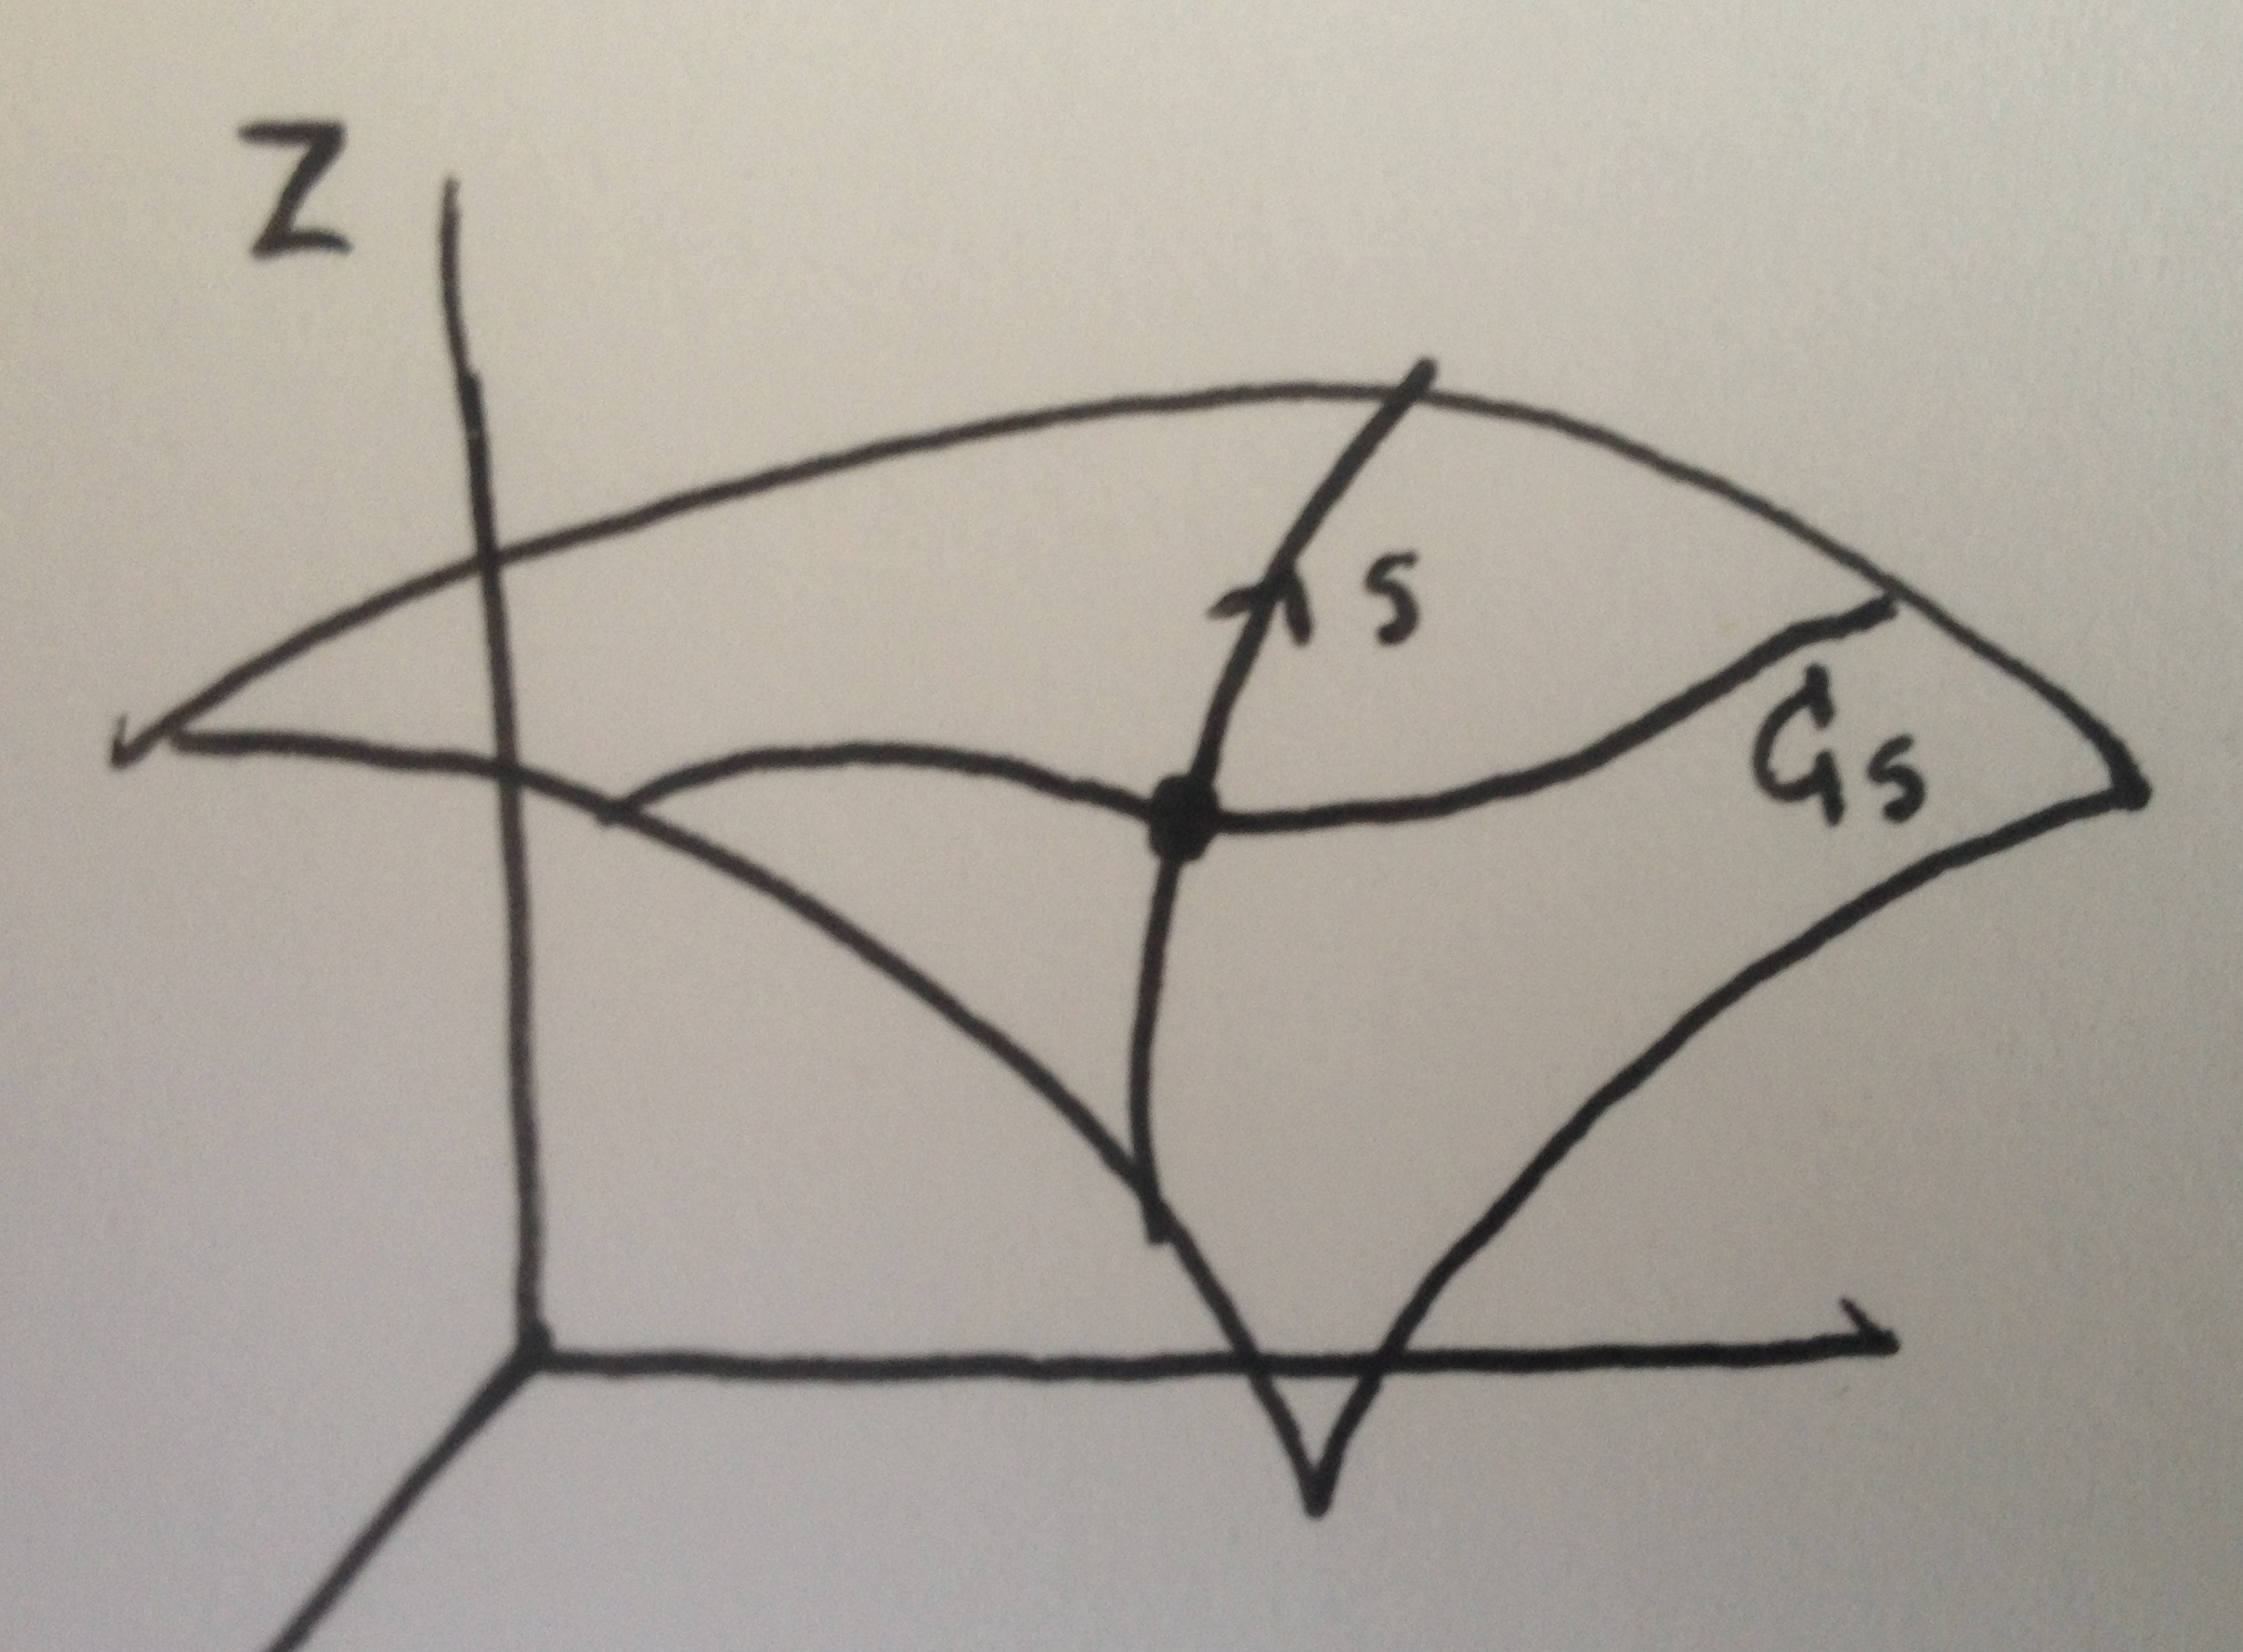
\includegraphics[width=3.0in]{moc_idea3.jpg}
\caption{Parameterized curve, with parameter $s$, going through initial data curve $\mathscr{C}_s$.}
\label{moc_idea3}
\end{figure}
\item[(iv)] For a fixed $\tau$, say $\tau=\tau_1$, the curve passing through the point $(x(\tau,0),y(\tau,0),u(\tau,0))$ on $\mathscr{C}_s$ can be considered as a parametric curve with parameter $s$. This idea is illustrated in Figure(\ref{mod_idea3}).
\item[(v)] A tangent vector to the parametric curve is: $\left< \frac{\partial x}{\partial s}, \frac{\partial y}{\partial s},  \frac{\partial u}{\partial s} \right>.$ 
\item[(vi)] The vector $<a,b,c>$ is also tangent to this curve!
\item[(vii)] Therefore $<a,b,c>$ and $\left< \frac{\partial x}{\partial s}, \frac{\partial y}{\partial s},  \frac{\partial u}{\partial s} \right>$ must be tangent to each other! E.g.,
$$\left< \frac{\partial x}{\partial s}, \frac{\partial y}{\partial s},  \frac{\partial u}{\partial s} \right> = k <a,b,c>,$$
where we can scale our parameter $s$ so such $k=1$ and we get the following system of ODEs
$$\left. \begin{array}{c}
\frac{\partial x}{\partial s} = a(x,y,u) \\
\frac{\partial y}{\partial s} = b(x,y,u) \\
\frac{\partial u}{\partial s} = c(x,y,u) \\
\end{array} \right\} \ \ \mbox{One parameter family of ODEs, called the \emph{characteristic equations} }.$$
Therefore we have
$$\frac{\partial u}{\partial s}  = \frac{\partial u}{\partial x} \frac{\partial x}{\partial s} + \frac{\partial u}{\partial y} \frac{\partial y}{\partial s} = a u_x + bu_y = c.$$

\item Finally, we have parameterized the initial data curve, $\mathscr{C}$, as 
\begin{align*}
x(\tau,0) &= f(\tau) \\
y(\tau,0) &= g(\tau) \\
u(\tau,0) &= u_0(\tau) \\
\end{align*}

The system of ODEs with these initial conditions yield a solution, 
\begin{align*}
x&=x(\tau,s) \\
y&=y(\tau,s) \\
u&=u(\tau,s) \\ 
\end{align*}
and upon inverting the transformation, if possible, i.e., solving for $\tau(x,y)$ and $s(x,y)$, we can arrive at our final solution, $$u(x,y) = u(\tau(x,y),s(x,y).$$
 
\end{itemize}

\end{enumerate}

%
% Mechanical Steps for Method of Characteristics!
%
\subsubsection{Mechanical Steps for the Method of Characteristics}

If the above description was not clear on the mechanistic approach, we will succinctly place the steps for the method of characteristics below. We again consider the Cauchy problem, $$a(x,y) u_x + b(x,y) u_y = c(x,y,u) \ \ \ \mbox{ with } \ \ \ u|_{\mathscr{C}} = u_0.$$

\begin{itemize}
\item[] {\bf{Step 1}}: Parameterize $\mathscr{C}$ in terms of $\tau$ and $s=0$,  $$\mathscr{C}: \left\{ \begin{array}{c} x=x(\tau,0) \\ y=y(\tau,0) \\ u=u(\tau,0) = u(x(\tau,0),y(\tau,0)) = u_0(\tau) \end{array} \right.$$
\item[] {\bf{Step 2}}: Solve the system of ODEs given by:
\begin{align*}
\frac{dx}{ds} &= a(x,y,u) \\
\frac{dy}{ds} &= b(x,y,u) \\
\frac{du}{ds}&= c(x,y,u) \\
\end{align*}
all subject to the initial conditions from Step 1. This then yields the following relation,
\begin{align*}
x&=x(\tau,s) \\
y&=y(\tau,s) \\
u&=u(\tau,s) \\
\end{align*}
\item[] {\bf{Step 3}}:  Solve for $s$ and $\tau$ in terms of $x$ and $y$, if possible*. Then $$u(x,y) = u(\tau(x,y),s(x,y)).$$ *Unfortunately, the coordinate transformations are not always invertible, or explicit in nature!

\end{itemize}


We will now present a few useful theorems regarding the method of characteristics. These all will be in the vein of the existence and uniqueness of solutions. 

\begin{theorem}
(\emph{Cauchy-Kowaleski Theorem}): Consider the Cauchy problem, $a(x,y,u) u_x + b(x,y,u) u_y - c(x,y,u)$ subject to a prescribed $u$ on a parametric curve, $\mathscr{C}: \left\{ \begin{array}{c} x = \bar{x}(\tau) \\ y=\bar{y}(\tau) \end{array} \right.,$ then we can let $u=u(\bar{x}(\tau),\bar{y}(\tau) )=u_0(\tau)$ for initial data. Suppose $a,b,c$ are continuously differentiable in a neighborhood of the initial data, i.e., the space curve $(\bar{x}(\tau), \bar{y}(\tau), u_0(\tau)).$ If 
$\left| \begin{array}{cc} a & b \\ X_\tau &Y_\tau \end{array}\right| \neq 0$ at all points on $\mathscr{C}$ (e.g., $\mathscr{C}$ is non-characteristic), then there exists a unique solution to the Cauchy problem in some neighborhood of the initial data curve, $\mathscr{C}.$
\end{theorem}

The following theorem can be used to identify when a Cauchy problem will have $\infty$-many solutions or no solution, based on the initial data.

\begin{theorem}
If $\left| \begin{array}{cc} a & b \\ X_\tau & Y_\tau \end{array}\right| = 0$ for all points on $\mathscr{C}$ (initial data curve itself is a characteristic), then the Cauchy problem has either $\infty-$many solutions or no-solution in a neighborhood of $\mathscr{C}.$
\end{theorem}

Throughout all of this analysis, we have employed use of the \emph{Implicit Function Theorem}, which tells us when we can invert a coordinate transformation. 
\begin{theorem}
(\emph{Implicit Function Theorem}) Consider $N$ equations with $N+M$ variables, $$F_k(x_1,x_2,\ldots,X_M,Y_1,\ldots,Y_N) = 0 \ \ \ \mbox{ for } \ \ \ k=1,2,\ldots,N,$$
or $${\bf{F}}({\bf{x}},{\bf{y}}) = 0.$$
We also assume each partial derivative of $F$is $C^1$ with respect to each $N+M$ variable. Furthermore we assume that the system of equations is satisfied at some point $P_0 = (x_1^0,\ldots,x_M^0,y_1^0,\ldots,y_N^0)$ with $$\left| \frac{\partial(F_1,\ldots,F_N)}{\partial(y_1,\ldots,y_N)} \right|_{P_0} \neq 0.$$
Then $\{y_k\}_{k=1}^{N}$ can be expressed as functions of $\{x_j\}_{j=1}^{M}$ in some neighborhood of $P_0$, i.e.,
\begin{align*}
y_1 = \phi_1(x_1,\ldots,x_M) \\
&\cdots \\
y_N = \phi_N(x_1,\ldots,x_M) \\
\end{align*}
or $${\bf{y}} = \vec{\phi}({\bf{x}}).$$
Moreover each $\{ \phi_k \}_{k=1}^{N}$ is $C^1$ with respect to each $\{x_j\}_{j=1}^{M}.$
\end{theorem}

The \emph{Implicit Function Theorem} in a nutshell, basically states that when we are given $\xi = \xi(x,y)$ and $\eta=\eta(x,y)$, we can write $x=x(\xi,\eta)$ and $y=y(\xi,eta)$ whenever $$\left| \begin{array}{cc} \xi_x & \xi_y \\ \eta_x & \eta_y \end{array} \right| \neq 0.$$

It is time to do an example! \emph{Let's boogey!}



%
% Method of Characteristics Example!
%
\subsubsection{Example: $x u_x - y u_y = 2xy^2$ with $u(x,1)=1+x^2$ on $0<x<1$}

Considering the PDE listed above. We will proceed with each of the mechanical steps we listed previously for solving a PDE using method of characteristics.

\begin{itemize}
\item[] {\bf{Step 1}}: Parameterize $\mathscr{C}$ with $\tau$ and $s=0$:
$$\mathscr{C}: \left. \begin{array}{c} x(\tau,0) = \tau \\ y(\tau,0) = 1 \end{array}\right\} \Rightarrow u(x(\tau,0),y(\tau,0))=u(\tau,1) = 1+\tau^2.$$

\item[] {\bf{Step 2}}: We setup the characteristics ODEs,
\begin{align*}
\frac{\partial x}{\partial s} &= x \\
\frac{\partial y}{\partial s} &= -y \\
\frac{\partial u}{\partial s} &= 2xy^2 = 2 \tau e^s e^{-2s} = 2\tau e^{-s}.
\end{align*}

Therefore solving the above system, we obtain
\begin{align*}
x &= Ke^{s}\Big|_{x(\tau,0)=\tau} \Rightarrow x=\tau e^s \\
y &= Ke^{s}\Big|_{y(\tau,0)=1} \Rightarrow y=e^{-s} \\
u(s) &= -2\tau e^{-s}+K\Big|_{u(\tau,0)=1+\tau^2} \Rightarrow u(\tau,s) = -2\tau e^{-s} + \tau^2 +2\tau + 1\\
\end{align*}

\item[] {\bf{Step 3}}: Inverting the transformations, we get 
\begin{align*}
x &= \tau e^s \Rightarrow \tau = xe^s = xy \\
y&= e^{-s} \Rightarrow s = -\ln(y),\ \ y>0 
\end{align*}

Hence we get our final solution as 
$$u(\tau,s) = -2\tau e^{-s} + \tau^2 +2\tau + 1 \Leftrightarrow  u(x,y) = -2xy^2 + 2xy + 1 + (xy)^2 = -2xy^2 + (xy+1)^2.$$

\end{itemize} $ $ \\ 

%
% General Method of Characteristics (for fully Nonlinear problem!)
%
\subsection{General Method of Characteristics for fully Nonlinear problems!}

In the above method of characteristics description, we have intentionally talked about the method of characteristics as used for \emph{quasi-linear} first-order PDEs. There is a more general version of the method of characteristics for fully nonlinear problems. We will describe the more general version now, but without much motivation. \\

The general method of characteristics in all its glory attempts to solve first-order PDEs of the form, $$F(x,y,u,u_x,u_y)=0,$$ with corresponding initial data $$\mathscr{C}: \left. \begin{array}{c} x=x(\tau) \\ y=y(\tau) \\ u(x(\tau),y(\tau)) = u(\tau) \end{array} \right\}.$$

First we use the following notation,
$$\left. \begin{array}{c}
p = u_x \\
q = u_y \\
\end{array} \right\} \Rightarrow \ \ \mbox{ standard notation}.$$

We will require that $u_x^2 + u_y^2 \neq 0,$ e.g., $p\neq 0$ when $q=0$ and vice-versa. We note that this mandates that the solution will not have any \emph{local} minima or maxima. Our governing PDE equation now takes the form, 

$$F(x,y,u,p,q) = 0.$$

Rolling through nonlinear method of characteristics rigmarole, which we do not expand upon here, we arrive at the following system of ODEs to solve,
\begin{align*}
\frac{dx}{ds} &= \frac{\partial F}{\partial p} \\
\frac{dy}{ds} &= \frac{\partial F}{\partial q} \\
\frac{du}{ds} & p\frac{\partial F}{\partial p} + q\frac{\partial F}{\partial q} \\
\frac{dp}{ds} &= -\left( \frac{\partial F}{\partial x} + p\frac{\partial F}{\partial u} \right) \\
\frac{dq}{ds} &= -\left( \frac{\partial F}{\partial y} + q\frac{\partial F}{\partial u} \right) \\
\end{align*}

with initial conditions $x(\tau,0)=x(\tau), y(\tau,0)=y(\tau), u(\tau,0)=u(\tau), p(\tau,0)=p(\tau), q(\tau,0)=q(\tau).$ For the initial conditions on $p(\tau)$ and $q(\tau)$, we use the conditions that

\begin{enumerate}
\item $F(x(\tau),y(\tau),u(\tau),p(\tau),q(\tau)) = 0$ \ \ \ (The differential equation is satisfied on the initial curve)
\item From $u_\tau = u_x x_\tau + u_y y_\tau$ on $\mathscr{C}$ we have that $u'(\tau) = p(\tau) x'(\tau) + q(\tau) y'(\tau).$
\end{enumerate}

Using those two bits of information we will be able to pick out the correct initial data for $p(\tau,0)$ and $q(\tau,0)$. We will leave you with just a few more notes on the general method of characteristics. 
\begin{enumerate}
\item Characteristics are still given by the level curves of $\tau(x,y)$.
\item If $F(x,y,u,p,q)$ is linear in $u_x$ and $u_y$, the above system reduces to the ``less-general" method of characteristics described previously
\item If $\left| \begin{array}{cc} x_\tau & x_s \\ y_tau & y_s \end{array}\right| = \left| \begin{array}{cc} x_\tau & F_p \\ y_tau & F_q \end{array}\right| = - \left| \begin{array}{cc} F_p & F_q \\ x_tau & y_\tau \end{array}\right| \neq 0$ on $\mathscr{C}$, then we are guaranteed a unique solution in some neighborhood of $\mathscr{C}.$
\end{enumerate}

Let's do an example for completeness!

%
% Nonlinear Method of Characteristics Example
%
\subsubsection{General Method of Characteristics Example: $u_x u_y = 1$ subject to $u(x,1) = 2\sqrt{x}$ for $x>0$}

First we write our first-order PDE in the form $$F(x,y,u,p,q) = u_x u_y -1 = pq -1,$$ with $p=u_x$ and $q=u_y$. We also note that $F_x=F_y=F_u=0,$ as well that $q = F_p$ and $p=F_q$. We then have the following system of ODEs to solve,
\begin{align*}
\frac{dx}{ds} &= F_p = q \\
\frac{dy}{ds} &= F_q = p \\
\frac{du}{ds} &= pF_p + qF_q = 2pq \\
\frac{dp}{ds} &= 0\\
\frac{dq}{ds} &= 0\\
\end{align*}
with initial conditions $x(\tau,0)=\tau, y(\tau,0)=1, u(\tau,0)=2\tau^{1/2}.$ Recall that on $\mathscr{C}$ the initial data is satisfied, hence we have 
\begin{itemize}
\item[(i)] $pq-1 = 0\Rightarrow p = \frac{1}{q} $ 
\item[(ii)] $u'(\tau) = pX'(\tau) + qY'(tau) \Rightarrow \tau^{1/2} = p(\tau,0)(1) + q(\tau,0)(0) = p$
\end{itemize}
on $\mathscr{C}$. Solving this system, we find that $$p(\tau,0) = \tau^{-1/2} \ \ \ \mbox{and} \ \ \ q(\tau,0)=\tau^{1/2}.$$

Now we have all the initial data we require and can proceed to solving the above system. Upon solving all these ODEs we find
\begin{align*}
\frac{dp}{ds} &= 0 \Rightarrow p(\tau,s) = C\Big|_{p(\tau,0)=\tau^{-1/2}} \Rightarrow p(\tau,s) = \tau^{-1/2} \\
\frac{dq}{ds} &= 0 \Rightarrow q(\tau,s) = C\Big|_{q(\tau,0)=\tau^{1/2}} \Rightarrow q(\tau,s) = \tau^{1/2} \\
\frac{dx}{ds} &= q \Rightarrow x(\tau,s) = \tau^{1/2}s + A(\tau)\Big|_{x(\tau,0)=\tau} \Rightarrow A(\tau) = \tau  \\
\frac{dy}{ds} &= p \Rightarrow y(\tau,s) = \tau^{-1/2}s + B(\tau)\Big|_{y(\tau,0)=1} \Rightarrow B(\tau) = 1  \\
\frac{du}{ds} &= 2pq \Rightarrow  u(\tau,s) = 2s + C(\tau)\Big|_{u(\tau,0)=2\tau^{1/2}} \Rightarrow C(\tau) = 2\tau^{1/2} \\
\end{align*}

and hence get
\begin{align*}
x(\tau,s) &= \tau^{1/2} s + \tau \\
y(\tau,s) &= \tau^{-1/2}s + 1\\
u(\tau,s) &= 2s+2\tau^{1/2}.\\
\end{align*}

Now we must try to transform back into $(x,y)$ coordinates from $(\tau,s)$. From the above relations, we see we can write 
$$\tau y = \tau^{1/2}+\tau = x,$$

and thereby $$x -\tau y = 0 \Rightarrow \tau = \frac{x}{y}.$$

Hence we find $$s = \left(\frac{x}{y}\right)^{1/2}(y-1),$$

and obtain as our final solution $$u(x,y) = 2\left(\frac{x}{y}\right)^{1/2}(y-1) + 2\left( \frac{x}{y} \right)^{1/2} = 2\sqrt{xy}.$$

We also state that the characteristics for the above problem are $\tau = \frac{x}{y} = constant.$

%%%%%%%%%%%%%%%%%%%%%%%%%%%%%%%%%%%%%
%
% SEPARATION OF VARIABLES
%
%%%%%%%%%%%%%%%%%%%%%%%%%%%%%%%%%%%%%

\subsection{Separation of Variables: For $2^{nd}$ order linear PDE (finite domains)}

In this section we will discuss a powerful method for finding solutions to linear PDE on finite domains. This is not the end-all, be-all technique for solving linear PDEs, but is very useful in areas from mechanics, electromagnetism, quantum mechanics, to economics. \\

We will show illustrate this method through an example.

\begin{itemize}
\item[] {\bf{Example}}: Heat Equation in $1d$ on a finite domain

Consider the following first-order linear constant coefficient, homogeneous PDE, $$u_t = \kappa u_{xx},$$ with associated boundary conditions $u(0,t)=u(1,t)=0,$ and initial value $u_0(x)=u(x,0) = f(x)$. Hence we consider the domain $x\in[0,1]$ and $t>0$. \\

We begin by assuming a solution of the form $$u(x,t)=X(x)T(t),$$ that is, $u(x,t)$ can be written as a product of two functions, one function with functional dependance only on $x$, and the other with functional dependence only on $t$. Performing that substitution we see 

$$u_t = \kappa u_{xx} \Rightarrow \frac{T'(t)}{T(t)} = \kappa \frac{X''(x)}{X(x)}.$$

From the above we see that since each side of the equation depends only on one independent variable, yet are equal for any values, that the quantity above must be equal to a constant, say $-\alpha^2.$ Hence we have 

$$\frac{T'(t)}{\kappa T(t)} =  \frac{X''(x)}{X(x)} = -\alpha^2.$$

We now have an eigenvalue in our problem...err...one more degree of freedom to work with! Before we get to that, we note that the boundary conditions are still to be obeyed, and are enforced via the $X(x)$ function, i.e., $ X(0)=X(1)=0.$ Now let's solve the above problem!\\

\begin{itemize}

%Solving T'(t) Equation
\item[] {\bf{Solving: $T'(t) = - \kappa\alpha^2 T(t)$}} \\ \\
We can solve this ODE simply by noticing its beautiful separable form, 
$$\frac{dT}{T} = -\kappa\alpha^2 dt,$$
and hence by simple integration obtain
$$T(t) = c_0 e^{-\kappa\alpha^2 t}.$$

We note that we did not get any information about the eigenvalue from solving this, nor can be use the initial value yet, since there is much spatial information to be learned! \\

\item[] {\bf{Solving: $X''(x) + \alpha^2 X(x) = 0.$}} \\ \\
In solving this equation we have to look at three cases, that is when $\alpha=0$, $\alpha^2 < 0$, and $\alpha^2>0.$\\
\begin{enumerate}

\item ${\bf{\alpha=0}}$: $$X'' = 0$$
and hence we have $$X(x) = cx+d.$$
Using the boundary conditions we see that $$X(0)=X(1)=0 \Rightarrow c=d=0,$$
and hence we only have the trivial solution.\\

\item ${\bf{\alpha^2 <0}}:$ $$X'' - \alpha^2 X = 0$$
Solving this we get in general that $$X(x) = c\sinh(\alpha x) + d\cosh(\alpha x).$$
Using the boundary conditions we see that 
\begin{align*}
X(0) &= d = 0\\
X(1) &= c\sinh(\alpha) = 0 \Rightarrow c = 0\\
\end{align*}
since we've assumed that $\alpha\neq0$ in this case. Hence we again only have the trivial solution present.\\

\item ${\bf{\alpha^2 > 0}}$: $$X'' + \alpha^2 X = 0$$

Solving the above ODE, we get $$X(x) = c\sin(\alpha x) + d\cos(\alpha x).$$

Now using the boundary conditions we find
\begin{align*}
X(0) &= d = 0 \\
X(1) &= c\sin(\alpha) = 0 \Rightarrow \alpha = n\pi \\
\end{align*}

where $n\in\mathbb{N}$. Therefore we find that our eigenvalue, $\lambda = \alpha^2 = n^2\pi^2.$ 

\end{enumerate}

\end{itemize}

Now we have both our solutions, $$u(x,t) = X(x)T(t) = c \sin(n\pi x) e^{-\kappa n^2 \pi^2 t};$$

however, we see that any positive integer value of $n$ gives us a different eigenvalue. It makes sense in fact we can use superposition to sum all of these possible solutions, each corresponding to a different eigenvalue, e.g.,

$$u(x,t) = \sum_{n=1}^{\infty} c_n  \sin(n\pi x) e^{-\kappa n^2 \pi^2 t}.$$

Note that we still have an infinite amount of coefficients $\{ c_j \}$ to find! Where, oh where, will we be able to find these? Welp, we haven't used the initial value for anything, yet. Let's start there!\\

Using the initial value, $u(x,0)=u_0(x) = f(x)$, we see that we have $$f(x) = \sum_{n=1}^{\infty} c_n \sin(n\pi x).$$ The above is simply a Fourier Series for $f(x)$! We can use the tricks and tools of the trade, i.e., orthogonality and completeness of the Fourier basis, to find $\{ c_n\}$.\\

Using Fourier Series, we note that we get

$$c_n = \frac{2}{L} \int_0^1 f(x) \sin(n\pi x) dx.$$

Therefore the final solution to our heat equation problem is $$u(x,t) =\frac{2}{L}  \sum_{n=1}^{\infty} \left[ \int_0^1 f(\tilde{x}) \sin(n\pi \tilde{x}) d\tilde{x} \right] \sin(n\pi x) \ e^{-\kappa n^2 \pi^2 t}.$$

$ $\\

%
% NON-HOMOGENOUS EXAMPLE
%
\item[] {\bf{Non-homogeneous Heat Equation}}

Consider the following first-order linear constant coefficient, non-homogeneous PDE, $$u_t = R + k u_{xx},$$ with associated boundary conditions, one of which is non-homogeneous, e.g., $u(0,t)=0$ and $u(1,t)=u_0$ for $t>0$, and initial value $u_0(x)=u(x,0) = f(x)$ for $0<x<1$. Hence we consider the domain $x\in[0,1]$ and $t>0$. \\

For problems of this type, we will begin by making a change of variables of the dependent variable, 
\begin{equation}
\label{nonhomo_change} u(x,t) = \psi(x,t) + \xi(x)
\end{equation}

Recal the boundary conditions in our new change of variables, 
\begin{align*}
u(0,t) &= \psi(0,t) + \xi(0) = 0 \\
u(1,t) &= \psi(1,t) + \xi(1) = 0 \\
\end{align*}

We will be able to put the non-homogeneous term all on the $\xi(x)$ function, provided we have $$\xi(0) = 0 \ \ \ \mbox{ and } \ \ \ \xi(1) = u_0.$$ In this case we then have translated homogeneous boundary conditions to $\psi(x,t)$ on $[0,1]$. We note that since $\xi(x)$ has no $t$ dependence, the initial conditions gets placed onto $\psi(x,t)$, i.e., $$u(x,0) = f(x) =  \psi(x,0) + \xi(x) \Rightarrow \psi(x,0) = f(x) - \xi(x).$$

Differentiating (\ref{nonhomo_change}) accordingly, we have
$$\frac{\partial^2 u}{\partial x^2} = \frac{\partial^2 \psi}{\partial x^2} + \xi''(x) \ \ \ \mbox{ and } \ \ \ \ \frac{\partial u}{\partial t} = \frac{\partial \psi}{\partial t}.$$

Therefore our model PDE becomes
$$k\frac{\partial^2 \psi}{\partial x^2} + k\xi'' + R = \frac{\partial\psi}{\partial t}.$$

The above equation will reduce to a homogeneous equation if we make the assumption that $$k\xi'' + R = 0.$$

Solving this (by two simple integration) gives $$\xi(x) = -\frac{R}{2k}x^2 + c_1 x + c_2.$$

Now making $\xi(x)$ obey the boundary conditions we set above gives
$$c_1 = \frac{R}{2k}+u_0 \ \ \ \ \mbox{ and } \ \ \ \ \ c_2 = 0.$$ 

Hence we find $$\xi(x) = -\frac{R}{2k}x^2 + \left[ \frac{R}{2k}+u_0\right]x.$$

Once we have $\xi(x)$, we can now set out to solve our homogeneous PDE given above, e.g., $$\psi_t  = k \psi_{xx},$$ with $\psi(0,t)=\psi(1,t) = 0$ for $t>0$ and $\psi(x,0) = f(x) - \xi(x).$ \\

It is clear that finding the solution to this PDE is identical to solving the homogeneous heat equation we previously have, but with differing initial condition. Rolling through the same separation of variables rigmarole, we find that 

$$\psi(x,t) = \sum_{n=1}^{\infty} c_n e^{-k n^2 \pi^2 t} \sin(n\pi x),$$

where we known the $\{c_j\}'s$ are given by orthogonality of the Fourier basis, 

$$c_n =  \frac{  \int_{0}^{1} \left[ f(x) + \xi(x) \right] \sin(n\pi x) dx }{\int_{0}^{1} \sin^2(n\pi x) dx } = 2 \int_{0}^{1} \left[ f(x) + \frac{R}{2k}x^2 - \left(\frac{R}{2k}+u_0\right) x \right] \sin(n\pi x) dx.$$

Therefore the solution to our original non-homogeneous PDE is given by
\begin{align*}
u(x,t) &= \psi(x,t) + \xi(x)\\ 
&=\sum_{n=1}^{\infty} \left[ \int_{0}^{1} \left[ f(\tilde{x}) + \frac{R}{2k}\tilde{x}^2 - \left(\frac{R}{2k}+u_0\right) \tilde{x} \right] \sin(n\pi \tilde{x}) d\tilde{x} \right] e^{-kn^2  \pi^2 t} \sin(n\pi x)   -  \frac{R}{2k}x^2 + \left[ \frac{R}{2k}+u_0\right]x.\\
\end{align*}

We note that the above solution is composed of two pieces, $\psi(x,t)$ and $\xi(x).$ We call $\xi(x)$ the \emph{steady-state} solution since we note that as $t\rightarrow\infty, \psi(x,t)\rightarrow 0$. We call $\psi(x,t)$ the \emph{transient} solution.

%
% Notes of Separation of Variables
%
\item[] {\bf{A few more notes on separation of variables}}: \\ \\

We will just say a few brief things about this method.
\begin{enumerate}
\item This methodology be used only for linear PDEs on finite domains
\item Such PDEs do not have to have constant coefficients; however, as long as the equation is separable and the resulting systems of ODEs leads to be of the \emph{Sturm-Liouville} flavor, you will be able to use this method
\item The example above easily goes through the mechanics and solutions to the wave equation and Laplace's Equation can be done analogously.
\item This methodology will work for higher order heat equations, wave equations, Laplace's equations, e.g., situations with more than two independent variables.
\item The change of variables, $u(x,t) = \psi(x,t) + \xi(x)$, will work for non-homogeneous problems involving Laplace's equation or the wave equation, as well.
\end{enumerate}


\end{itemize} %ENDS HEAT EQUATION EXAMPLE


%%%%%%%%%%%%%%%%%%%%%%%%%%%%%%%%%%%
%
% INTEGRAL TRANSFORMs for PDE
%
%%%%%%%%%%%%%%%%%%%%%%%%%%%%%%%%%%%

\subsection{Integral Transforms: Linear PDEs on $\mathbb{R}\ (or \mathbb{R}^n)$}

In this section we will show how to use the Fourier Transform, Laplace Transform, and alike methods for solving some linear PDEs. In general for linear PDEs on $\mathbb{R}$, we will use the \emph{Fourier Transform}, while for variables defined on $[0,\infty)$ we will use the \emph{Laplace Transform}. We will begin with a brief overview of the \emph{Fourier Transform}

%
% FOURIER TRANSFORM
%
\subsubsection{The Fourier Transform}

We begin with the definition of the Fourier Transform,
\begin{equation}
\label{Fourier_Transform} \mathscr{F}\{f(x)\}(k) = F(k) =  \int_{-\infty}^{\infty} f(x) e^{-ikx} dx.
\end{equation}

We note that not every function $f(x)$ will have a Fourier Transform; however, a sufficient condition for a function to have one (i.e., the above integral converges) is that $f(x)$ is square-integrable, e.g., $$||f(x)||^2 = \int_{\mathbb{R}} |f(x)|^2 dx = \mbox{ a constant}.$$ 

If $f(x)$ is also continuous as well, then the Inverse Fourier Transform should exist, and we have the inversion formula 
\begin{equation}
\label{Inverse_Fourier_Transform} f(x) =\frac{1}{2\pi} \mathscr{F}^{-1}\{ F(k) \}(x) = \int_{\mathbb{R}} F(k) e^{ikx} dk.
\end{equation}

We will now discuss a few properties of the Fourier Transform.

\begin{enumerate}

%Linearity
\item {\bf{Linearity}}: \\ \\

Like the Laplace Transform, linearity holds in the Fourier Transform. If it didn't, it probably wouldn't be worth a second glance, after-all.
$$\mathscr{F}\{ c_1 f_1(x) + c_2 f_2(x) \} = c_1 \mathscr{F}\{f_1(x)\} + c_2\mathscr{F}\{f_2(x) \} = c_1F_1(k) + c_2F_2(k),$$

where $\{c_1,c_2\}\in\mathbb{C}.$ 

%Translation
\item {\bf{Translations}}: \\ \\

We also have the following translational property,
\begin{align*}
\mathscr{F}\{ f(x-a)\} &= \int_{\mathbb{R}} f(x-a) e^{-ikx} dx \\
&= \int_{\mathbb{R}} f(u) e^{-ik(u+a)} du \\
&= e^{-ika} \int_{\mathbb{R}} f(u) e^{-iku} du \\
&= e^{-ika} F(k)\\
\end{align*}

Hence we have $$\mathscr{F}\{ f(x-a)\} =e^{-ika} F(k).$$

%SCALING
\item {\bf{Scaling}}: \\ \\
The following scaling property also holds
$$\mathscr{F}\{ f(cx) \} = \frac{ F\left( \frac{k}{c} \right)}{|c|}.$$

%CONVOLUTION
\item {\bf{Convolution}}: \\ \\ 

The Fourier Transform of a convolution of two functions, $f_1(x)$ and $f_2(x)$, has an elegant (and convenient!) form,

$$\mathscr{F}\{ f_1(x)\ast f_2(x) \} = F_1(K) F_2(k).$$

%MODULATION
\item {\bf{Modulation}}: \\ \\

The Fourier Transform of a modulation (product) of functions is given by

$$\mathscr{F}\{ f_1(x)f_2(x)  \} = F_1(x) \ast F_2(x).$$

%PARSEVAL'S THEOREM
\item {\bf{Parseval's Theorem}}: \\ \\

$$\int_{\mathbb{R}} | f(x) |^2 dx = \int_{\mathbb{R}} | F(k) |^2 dk,$$ or equivalently

$$||F(k)||^2 = \frac{1}{2\pi} ||f(x)||^2.$$

This identity becomes especially useful when doing stability analysis of numerical methods involving finite differencing for the solutions of PDEs.

%Duality
\item {\bf{Duality}}: \\ \\

Suppose $f(x)$ has Fourier Transform $F(k)$. Then we immediately know the Fourier Transform of the function $F(x)$! This is known as the duality property of the Fourier Transform, as seen below

$$\mathscr{F}\{ F(x) \} = 2\pi f(-k).$$

%Derivatives!
\item {\bf{Derivatives!}}:\\ \\

When we take the Fourier Transform of a derivative, we will simply use our good friend, integration by parts, to help us out. Knowing that our function is square-integrable is what will allow us to drop terms. Let's check it out

\begin{align*}
\mathscr{F}\left\{\frac{df}{dx} \right\} &= int_{\mathbb{R}} \frac{df}{dx} e^{-ikx} dx \\
&= f(x)  e^{-ikx} \Big|_{\mathbb{R}} +  \int (-ik) f(x) e^{-ikx} dx \\
&= (-ik) \int_{\mathbb{R}} f(x) e^{-ikx} dx \\
&= (-ik) F(k)
\end{align*}

Therefore we find that $$\mathscr{F}\left\{\frac{df}{dx} \right\}  = (-ik) F(k).$$

We can continue analogously for higher order derivatives, and by induction, we get the following relation

$$\mathscr{F}\left\{ \frac{d^n f}{dx^n}  \right\} = (-ik)^n F(k).$$

%
% Derivative of FT of Non-Transformed Variable
%
\item {\bf{Derivatives with respect to non-transformed variables}}:\\ \\

Consider taking the Fourier Transform \emph{with respect to} $x$ of $\frac{\partial u}{\partial t}.$ We will see since $t$ is a dummy-type variable and our integration does not depend on it, it makes sense we will be able to pull the derivative operator with respect to $t$ out of the integral. Let's check it out rigorously,

\begin{align*}
\mathscr{F}\left\{ \frac{\partial u}{\partial t} \right\} &= \int_{\mathbb{R}} u_t(x,t) e^{-ikx} dx \\
&= \int_{\mathbb{R}} \frac{ u(x,t+\Delta t) - u(x,t) }{\Delta t} e^{-ikx} dx \\
&= \lim_{\Delta t\rightarrow 0} \frac{1}{\Delta t} \left[ \int_{\mathbb{R}} u(x,t+\Delta t) e^{-ikx} dx - \int_{\mathbb{R}} u(x,t) e^{-ikx} dx  \right] \\
&= \lim_{\Delta t\rightarrow 0} \frac{1}{\Delta t} \left[ U(k,t+\Delta t) - U(k,t) \right] \\
&= \frac{\partial}{\partial t} U(k,t)\\
\end{align*}

Naturally this result holds for higher order derivatives, i.e.,
$$\mathscr{F}\left\{\frac{\partial^n u}{\partial t^n}  \right\} = \frac{\partial}{\partial t^n} U(k,t).$$
\end{enumerate}

Now let's proceed to solve a PDE using Fourier Transform! 


%
% USING FT TO SOLVE WAVE EQUATION
%
\subsection{Fourier Transform to Solve a PDE}

Consider the following hyperbolic equation, e.g., in this case the \emph{wave equation},
$$u_{tt} = c^2 u_{xx},$$ with $u\rightarrow0$ as $|x|\rightarrow \infty$ and for $t>0$. We begin by taking the Fourier Transform of both sides of this equation, 

$$\int_{\mathbb{R}} u_{tt} e^{-ikx} dx = \int_{\mathbb{R}} c^2 u_{xx} dx.$$

From properties of the Fourier Transform we saw in the previous section, we see that this gives us 

$$\frac{\partial^2 }{\partial t^2} U(k,t) = c^2 (-ik)^2 U(k,t) = -c^2k^2 U(k,t)$$

Hence taking the Fourier Transform has transformed our PDE into an ODE. We now just consider $k$ as some fixed parameter, and see our problem is reduced to a constant coefficient ,homogeneous linear ODE. We can easily solve this ODE using familiar methods from basic ODE theory. Let $$U(k,t) = e^{\alpha t},$$

and upon substituting we see we get the solution

$$U(k,t) = C_1(k)e^{-ickt} + C_2(k) e^{ickt},$$

where $C_1(k)$ and $C_2(k)$ are functions strictly of $k$ and will be able to be found via initial conditions. We note that when $k=0$, the ODE becomes singular and we instead have to solve $U_{tt} = 0$, which leads to the trivial solution when mandating that the solution remain physical. \\

Now to recover the solution we care about in physical space, i.e., $u(x,t)$, we need to use the Inverse Fourier Transform to transform back appropriately. Doing this we find
\begin{align*}
\mathscr{F}^{-1}\{ U(k,t)  \} &= \frac{1}{2\pi} \int_{\mathbb{R}} U(k,t) e^{-ikx} dk\\
&= \frac{1}{2\pi} \int_{\mathbb{R}} \left[ C_1(k) e^{-ickt} + C_2(k) e^{ickt} \right] e^{ikx} dk\\
&= \frac{1}{2\pi} \left[ \int_{\mathbb{R}} C_1(k) e^{ik(x-ct)} dk + \int_{\mathbb{R}} C_2(k) e^{ik(x+ct)} dk  \right] \\
&= c_1(x-ct) + c_2(x+ct) 
\end{align*}

where $C_1(k,t) = \int_{\mathbb{R}} c_1(x,t) e^{-ikx} dx$ and $C_2(k,t) = \int_{\mathbb{R}} c_2(x,t) e^{-ikx} dx$ and hence their Inverse Fourier Transforms are used above. We note that this solution is called the \emph{D'Alembert} solution, which describes wave phenomena, where one wave packet moves to the right, $c_1(x-ct)$, and one wave packet moves to the left, $c_2(x+ct).$


%
% USING LAPLACE TRANSFORM TO SOLVE WAVE EQUATION
%
\subsection{Laplace Transform to Solve a PDE}

Consider the following wave equation, $$u_{tt}=c^2 u_{xx},$$
with boundary conditions $u(0,t)=u(1,t) = 0$ for $t>0$, and initial values $u(x,0)=0$ and $u_t(x,0) = \sin(\pi x)$ on $0<x<1$. We note that the spatial domain is finite, making us consider another method besides Fourier Transforms. We could, of course, notice the equation is separable, and use separation of variables, but we already had our fun with those, and yurn to use integral transforms! \\

Since the variable $t$ is defined for $t\in[0,\infty),$ we can use Laplace Transforms to transform the equation in this variable. Taking the Laplace Transform of both sides of the equation gives

\begin{align*}
\mathscr{L}\left\{ \frac{\partial^2 u}{\partial t^2} \right\} &= \mathscr{L}\left\{ c^2 \frac{\partial^2 u}{\partial x^2} \right\} \\
\int_{0}^\infty u_{tt} e^{-st} dt &= \int_{0}^\infty c^2 u_{xx} e^{-st} dt \\
s^2 U(x,s) - s u(x,0) - u_t(x,0) &= c^2 \frac{ d^2 U}{dx^2} 
\end{align*}

and hence we have the following ODE to solve

$$U_xx - s^2 U = s u(x,0) + u_t(x,0) = \sin(\pi x),$$

by substituting our initial data. However, before we go further we recognize that the boundary conditions are functions of $t$ and hence themselves must be transformed as well,
\begin{align*}
\mathscr{L}\{ u(0,t)  \} &=  \mathscr{L}\{ 0 \} = 0 = U(0,t) \\
\mathscr{L}\{ u(1,t)  \} &=  \mathscr{L}\{ 0 \} = 0 = U(1,t).
\end{align*}

Now we have the appropriate boundary conditions to use when solve the ODE in the transformed space. Proceeding with the solution, we first solve the homogeneous problem, i.e., $U_xx - s^2 U = 0$, to get the complementary solution and find $$U_C(x,s) = c_1 \cosh(sx) + c_2 \sinh(sx),$$

since $s>0$ in the Laplace Transform. However, using the boundary conditions, we find that $c_1 = c_2 = 0.$ Onwards to solve for the particular solution, we can use the method of undetermined coefficients (or variation of parameters if you're really that bored), starting with an initial guess for the particular solution as $$U_P(x,s) = A \cos(\pi x) + B\sin(\pi x).$$

Substituting this into the ODE, we find that $A=0$ and $B=\frac{1}{s^2+\pi^2}.$ Therefore our solution is:

$$U(x,s) = U_C(x,s) + U_P(x,s) = \frac{1}{s^2+\pi^2} \sin(\pi x).$$

Now we must transform back into physical space, 
\begin{align*}
u(x,t) &= \mathscr{L}^{-1}\left\{ U(x,s)  \right\} \\
& =  \mathscr{L}^{-1}\left\{  \frac{1}{s^2+\pi^2} \sin(\pi x) \right\} \\
& = \frac{1}{\pi}  \mathscr{L}^{-1}\left\{  \frac{\pi}{s^2+\pi^2} \sin(\pi x) \right\} \\
&= \frac{1}{\pi} \sin(\pi x) \sin(\pi t).
\end{align*}




%%%%%%%%%%%%%%%%%%%%%%%%%%%%%%%%
%
% SIMILARITY SOLUTIONS
%
%%%%%%%%%%%%%%%%%%%%%%%%%%%%%%%%

\subsection{Similarity Solutions!}

Similar transformations can help give a lot of information about certain PDEs; however, we can also use them to cook up solutions when some of (or all) of the independent variables appear through certain groupings, rather than independently. Consider the following example involving the 2D heat equation.

\begin{enumerate}
\item {\bf{2D Heat Equation}} \\ \\
For example, if we consider the heat equation $$u_t = k(u_{xx} + u_{yy},$$ we can search for solutions that depend on $x$ and $y$ through the grouping, $$r(x,y) = \sqrt{x^2+y^2}, $$ e.g.,

$$u(x,y,t) \rightarrow u(r(x,y),t) = u(r,t),$$ and $$u_x = u_r r_x \Rightarrow u_{xx} = u_{rr} r_x^2 + u_r r_{xx} = u_{rr}\frac{x^2}{r^2} + u_r \frac{y^2}{r^3},$$
and analogously for $u_{yy}$ we get, $$u_{yy} = u_{rr}\frac{y^2}{r^2} + u_r \frac{x^2}{r^3},$$
and hence $$u_{xx}+u_{yy} = u_{rr}+\frac{1}{r} u_r.$$ Doing these substitutions leads to the radially symmetric heat equation, $$u_t = k\left[ u_{rr} + \frac{1}{r} u_r\right].$$

\item {\bf{1D Wave Equation}} \\ \\
Consider $$u_t + au_x = 0.$$ We will search for solutions of the form $u=u(\xi(x,t))$ where $\xi(x,t)=x-at.$ Performing the necessary derivatives, we get
$$u_t = u_\xi xi_t = -a u_\xi \ \ \ \mbox{ and } \ \ \ u_x = u_\xi \xi_x = u_\xi.$$ Therefore substituting these into the wave equation above we find
\begin{align*}
u_t + au_x &= 0 \\ 
(-au_\xi ) + a(u_\xi) &= 0\\
0&= 0 \Rightarrow \ \ \mbox{all differentiable functions of } \xi \mbox{ satisfy the PDE}.\\
\end{align*}

Therefore we find our solutions take the form $$u(x,t) = f(x-at).$$

We now make the claim that no solutions are lost by this similarity transformation. To see this we will find the solution using this idea of similarity transformation! We will make the full coordinate transformation, 
$$\xi = x-at \ \ \ \mbox{ and } \ \ \ \eta = \eta(x,t).$$
Recall from the Implicit Function Theorem if $$\left| \begin{array}{cc} \xi_x & \xi_t \\ \eta_x & \eta_t \end{array} \right| = \left| \begin{array}{cc} 1 & -a \\ \eta_x & \eta_t \end{array} \right| = \eta_t - a\eta_x \neq 0,$$ then we have an invertible transformation. We just need $\eta(x,t)$ to satisfy the above.

Performing the necessary derivatives we find
\begin{align*}
u_t &= u_\xi \xi_t + u_\eta \eta_t = -a u_\xi + u_\eta \eta_t \\
u_x &= u_\xi \xi_x + u_\eta \eta_x = u_\xi +u_\eta \eta_x \\
\end{align*}

Substituting these into our governing PDE gives
\begin{align*}
u_t + au_x &= -au_\xi + u_\eta \eta_t + au_\xi + au_\eta \eta_x \\
&= u_\eta (\eta_t + a\eta_x) =0.
\end{align*}

Hence we require that $u_\eta=0$ so that our coordinate transformation remains invertible, by our determinant above. Solving this ODE, we find $u(\xi,\eta)=C(\xi),$

and therefore $$u(x,t) = C(x-at).$$

\item {\bf{1D Heat Equation}} \\ \\

Consider the $1D$ heat equation, $$u_t =  k u_{xx}.$$ We wish to use similarity transformations to try to cook up a solution. In general we will look for solutions with groupings of the independent variables, such as $\xi(x,t) = x^\alpha y^\beta,$ where $\alpha,\beta\neq 0.$ We then assume a solution of the form $$u(x,t) = u(\xi(x,t)).$$

We proceed with performing the necessary differentiations,
\begin{align*}
u_t &= u_\xi \xi_t = u_\xi \beta x^\alpha t^{\beta-1} = u_\xi \beta \frac{\xi}{t} \\
u_x&= u_\xi \xi_x = u_\xi \alpha x^{\alpha-1} t^\beta = u_\xi \alpha \frac{\xi}{x}\\
\end{align*}

and hence
\begin{align*}
u_{xx} = u_{\xi\xi} \xi_x^2 + u_\xi \xi_{xx} &= u_{\xi\xi} \alpha^2 \frac{\xi^2}{x^2} + u_\xi \alpha(\alpha-1) x^{\alpha-2}t^\beta \\
&= u_{\xi\xi}\alpha^2 \frac{\xi^2}{x^2} + u_\xi \alpha(\alpha-1) \frac{\xi}{x^2}.\\
\end{align*}
  
Our governing equations then becomes $$u_t = ku_{xx} \ \Rightarrow \ u_{\xi}\beta\frac{\xi}{t} = k\left[ u_{\xi\xi} \alpha^2 \frac{\xi^2}{x^2} + u_\xi\alpha(\alpha-1)\frac{\xi}{x^2}  \right],$$

and thereby
$$u_\xi \beta\xi \frac{x^2}{t} = k\left[ u_{\xi\xi} \alpha^2 \xi^2 + u_\xi \alpha(\alpha-1)\xi  \right].$$

Now in the vein of similarity solutions, we want to try to get rid (or group) all the $x$'s and $t$'s. In the above equation, we must let the quantity, $\frac{x^2}{t}$ be some power of $\xi$ if the transformation is successful. Now we let $$\xi^p = \frac{x^2}{t},$$ and hence get that $$(x^\alpha y^\beta)^p = \frac{x^2}{t} \Rightarrow 2=\alpha p \ \ \ \mbox{ and } \ \ \ -1 = \beta p,$$ and therefore $$\beta = -\frac{\alpha}{2}.$$

We only have the one condition above and $\alpha$ can be chosen at our discretion. Let's let $\alpha=1$ (that seems nice). It also kills a term in our governing equation. We now have $\beta = -\frac{1}{2} \Rightarrow \xi(x,y) = \frac{x}{\sqrt{t}}.$ Our governing equation then becomes,
$$-\frac{1}{2} u_{\xi} \xi^3 = k u_{\xi\xi} \xi^2 \ \ \Rightarrow \ \ -\frac{\xi}{2k} u_{\xi} = u_{\xi\xi} \ \ \Rightarrow \ \ u_{\xi\xi} + \frac{\xi}{2k} u_{\xi} = 0.$$

We can now integrate this equation with respect to $\xi$, to get $$u_{\xi} = Ae^{-\frac{\xi^2}{4k}},$$ and by integrating once again, we get $$u(\xi) - u(0) = \int_{0}^{\xi} A e^{-\frac{s^2}{4k}} ds.$$

If the above doesn't immediately scream \emph{error function} to you, we will introduce you to that friendly function now. 

\begin{definition}
The \emph{error function} is defined as $$\erf(z) = \frac{2}{\pi} \int_{0}^z e^{-t^2} dt,$$ with properties $$\erf(\pm\infty) = \pm 1 \ \ \ \mbox{and} \ \ \ \erf(x) \ \mbox{is odd}.$$
\end{definition}

We can now write our solution in terms of the error function as 
\begin{align*}
u(\xi) - u(0) &= A \int_{0}^{\xi} e^{-\frac{s^2}{4k}} ds \\
&= \int_0^{\frac{\xi}{2\sqrt{k}}} e^{-t^2} 2\sqrt{k} dt \\
&= \tilde{A} \frac{2}{\pi} \int_0^{\frac{\xi}{2\sqrt{k}}} e^{-t^2} dt \\
\end{align*}

and then we get $$u(\xi) = u_0 + \tilde{A} \erf\left( \frac{\xi}{2\sqrt{k}}  \right),$$
and finally upon substituting back into $(x,t)$ coordinates, using $\xi = \frac{x^2}{t},$ $$u(x,t) = u_0 + \tilde{A} \erf\left( \frac{x}{2\sqrt{kt}} \right).$$

\end{enumerate}


%%%%%%%%%%%%%%%%%%%%%%%%%%%%%%%%
%
% METHOD OF IMAGES
%
%%%%%%%%%%%%%%%%%%%%%%%%%%%%%%%%

\subsection{Method of Images}

The method of images is a technique used for solving certain differential equations, where the domain of a certain problem is extended by the addition of a complementary domain, usually with some respective symmetrical form to the original, in which certain boundary conditions are instantly satisfied, and hence the solution to the original problem is facilitated. It is commonly used in \emph{electrostatics}, where an array of point charges are located in the vicinity of a conducting or insulating surface, and the corresponding electric field is desired.  Besides electrostatics, it is analogous to methods used in highly symmetric optics problems. We note that this method heavily depends on uniqueness\\

We will perform two examples of the method of images to illustrate this idea. This section will also require some basic electrostatic a priori physics knowledge. Well, either that or a basic understanding of fundamental solutions of elliptic problems...whichever you'd prefer! \\

%
% Single Point Charge: Infinite Conducting Plate
%
\subsubsection{Example: Infinite conducting plate with single point charge}

\begin{figure}[h!]
\centering
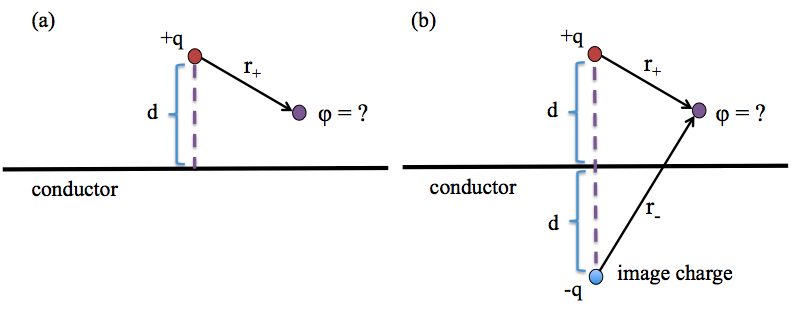
\includegraphics[width=5.5in]{moi_geo1.png}
\caption{(a) Single point source (charge) above an infinitely long conducting surface. (b) The same geometry, but with a virtual source point (with opposite charge) located symmetrically across the conducting plane.}
\label{MOI_geo1}
\end{figure}

We consider a single point source (charge) in the upper half plane, where it is placed above an infinitely long conducting surface. This is illustrated in Figure(\ref{MOI_geo1}a). We are interested in what the \emph{electric field}, or just vector field, $\phi$, looks like at another point in the plane. The governing problem is that of \emph{Poisson} problem, an elliptic PDE, 
$$\Delta \phi = -\frac{q}{\epsilon_0} \delta({\bf{r}} - {\bf{r}}_0),$$ where ${\bf{r}}_0 = d \hat{z},$ the location of the point source, $+q$, and $\phi$ is the potential associated with such point source. We note that for any non-homogeneous differential equation, we will have both a complementary solution and particular solution. Our only boundary condition is that on the conducting surface, say at $z=0$, the potential is zero. \\

This is where the intuition behind the method of images is beautiful. Rather than look for a particular solution, say $\phi_+$, and a complementary solution, $\phi_{-}$, to the equations $$\Delta \phi_+ = -\frac{q}{\epsilon_0} \delta({\bf{r}}-{\bf{r}}_0) \  \ \  \mbox{ and } \ \ \ \Delta \phi_{-}= 0,$$ respectively, we will try to cook up a solution that satisfies the boundary condition at $z=0$ using knowledge of the fundamental solution of such elliptic operator, e.g., $\Delta$ in $2D$.\\

We note that the general potential for such an operator is given by $\phi = \frac{k}{r}$, where $k$ is a constant that is determined by the physics in the underlying problem. Here $k=\frac{\pm q}{4\pi\epsilon_0},$ where $\pm q$ depends on which source term you are considering. If we need combine these two solutions, we note we can satisfy the boundary condition at $z=0$, if we place a point charge of equal and opposite sign at the mirror image of the other charge below the plane. This is seen in Figure(\ref{MOI_geo1}b).\\

\emph{Note} that below the plane is not even in the original domain of the problem, hence when we consider the Poisson-type problem for it's source charge, we find $$\Delta \phi_{-} = \delta( {\bf{r}}-{\bf{r}}_{im}) = 0,$$ where ${\bf{r}}_{im} = -d \hat{z},$ since ${\bf{r}}_{im}$ is not in the domain of the problem at hand.\\

Therefore the solution to this Poisson problem is $$\phi = \phi_{+} + \phi_{-} = \frac{1}{4\pi\epsilon_0} \left[  \frac{q}{r_+} + \frac{-q}{r_{-}}  \right] =\frac{1}{4\pi\epsilon_0} \left[ \frac{q}{\sqrt{x^2 + (z-d)^2 }} + \frac{-q}{\sqrt{x^2 + (z+d)^2}}  \right] $$


%
% Subsection: Example: Point Charge and Grounded Sphere
%
\subsection{Example: Point Charge and a Grounded Sphere}

\begin{figure}[h!]
\centering
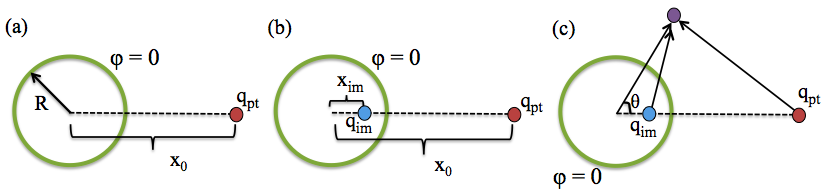
\includegraphics[width=6.25in]{moi_geo2.png}
\caption{(a) Single point source of charge $q_{pt}$ outside a grounded sphere. (b) The same geometry, but with a virtual source point (with differing) located inside the grounded sphere at an unknown location, $x_{im}$. (c) Illustrating the influence from both the point charge and image point charge on a point outside the sphere.}
\label{MOI_geo2}
\end{figure}

Consider the problem of a point charge outside of a grounded sphere.  Since the sphere is grounded, we need the potential to be equal to zero on the entire sphere. This is our boundary condition. To setup the geometry, say the point charge is a distance $x_0$ away from the sphere of radius, $R$.  For simplicity, we will also center the sphere about the origin. This is shown below in Figure(\ref{MOI_geo2})(a). \\ 

In order to find the potential everywhere using the method of images, we must need to find the location of the virtual point charge, such that the boundary condition on the sphere is satisfied. To do this, we make the hypothesis, that to preserve symmetry, this image point should be placed somewhere along the $x-axis$, and moreover, to satisfy that $\phi = 0$ along the sphere, intuition suggests this point will need to be inside the sphere.\\

Rather than try to calculate the potentials of both these points to satisfy the boundary condition along the entire sphere, we consider trying to satisfy the boundary condition at two points along the $x$-axis, namely $(R,0)$ and $(-R,0)$, i.e.,

\begin{itemize}
\item At $(R,0)$, $\phi = 0$
\item At $(-R,0)$, $\phi=0.$
\end{itemize}

If this doesn't make sense why we only consider these two points, we have somewhat pulled a fast one. Well, not really. We are just using what scientists call \emph{hindsight}, err I mean, foresight when thinking about a problem. The motivation is as follows. We note that using the fundamental solution for $\Delta\phi=0$ in radial coordinates in $2-D$ for electrostatics problems, we will have two unknowns when placing the image point - the location along the $x$-axis and the strength of the charge. The train of thought then follows that by using as much symmetry as possible, if we are able to write a system of two equations and two unknowns, we then can get all the information we need for finding the true solution. 

Therefore from those two (more specific) boundary conditions, we get
\begin{align*}
\phi \Big|_{(x,y)=(R,0)} = 0 &=\frac{1}{4\pi\epsilon_0} \left[ \frac{q_{pt}}{(x_0 - R)} +  \frac{q_{im}}{(R-x_{im})} \right] \\
\phi\Big |_{(x,y)=(-R,0)} = 0  &= \frac{1}{4\pi\epsilon_0}\left[ \frac{q_{pt}}{(x_0 + R)}  +  \frac{q_{im}}{(x_{im}+R)} \right].
\end{align*}

Solving the above system of two equations and two unknowns yields, 
$$x_{im} = \frac{R^2}{x_0} \ \ \ \mbox{ and } \ \ \ q_{im} = \frac{-q_{pt} R}{x_0}.$$

Now to calculate the potential of any point outside the sphere, $(r,\theta,\phi)$, we find 
$$\phi(r,\theta,\phi) = \phi_{pt}\Big |_{(r,\theta,\phi)} + \phi_{im}\Big|_{(r,\theta,\phi)} = \frac{1}{4\pi\epsilon_0} \left[ \frac{q_{pt}}{\sqrt{r^2+x_0^2- 2rx_0\cos\theta}} + \frac{-\frac{q_{pt}R}{x_0}}{\sqrt{r^2+\frac{R^4}{x_0^2} - 2r\frac{R^2}{x_0}\cos\theta}}  \right].$$

At this junction, you may be wondering whether or not the above solution truly satisfies the boundary condition on the entire sphere. Well, the nice thing about PDEs (and differential equations in general) is we can always check out solution. (\emph{If time permits on tests, of course...})\\

We first consider an arbitrary point on the sphere, say distances from charges $q_{pt}$ and $q_{im}$ of
$$d_{pt} = \sqrt{R^2+x_0^2 -2Rx_0\cos\theta} \ \ \ \mbox{and} \ \ \ d_{im} = \sqrt{R^2+\left(\frac{R^2}{x_0}\right) - 2R\left(\frac{R^2}{x_0}\right)\cos\theta},$$

respectively. Now the potential on the surface of the sphere is given by
\begin{align*}
\phi \Big|_{r=R} &= \frac{1}{4\pi\epsilon_0}\left[ \frac{q_{pt}}{d_{pt}} + \frac{q_{im}}{d_{im}}  \right]  \\
&= \frac{1}{4\pi\epsilon_0} \left[ \frac{q_{pt}}{\sqrt{R^2+x_0^2- 2Rx_0\cos\theta}} + \frac{-\frac{q_{pt}R}{x_0}}{\sqrt{R^2+\frac{R^4}{x_0^2} - 2R\frac{R^2}{x_0}\cos\theta}}  \right] \\
&= \frac{1}{4\pi\epsilon_0} \left[ \frac{q_{pt}}{\sqrt{R^2+x_0^2- 2Rx_0\cos\theta}} + \frac{q_{pt}}{\sqrt{ \frac{x_0^2}{R^2}\left( R^2+\frac{R^4}{x_0^2} - 2\frac{R^3}{x_0}\cos\theta  \right)           } }  \right] \\
&= \frac{1}{4\pi\epsilon_0} \left[ \frac{q_{pt}}{\sqrt{R^2+x_0^2- 2Rx_0\cos\theta}} - \frac{q_{pt}}{\sqrt{x_0^2+R^2 -2Rx_0\cos\theta}} \right] \\
&= 0.
\end{align*}

Hence our solution checks out!
